\documentclass[]{article}
\usepackage{lmodern}
\usepackage{amssymb,amsmath}
\usepackage{ifxetex,ifluatex}
\usepackage{fixltx2e} % provides \textsubscript
\ifnum 0\ifxetex 1\fi\ifluatex 1\fi=0 % if pdftex
  \usepackage[T1]{fontenc}
  \usepackage[utf8]{inputenc}
\else % if luatex or xelatex
  \ifxetex
    \usepackage{mathspec}
  \else
    \usepackage{fontspec}
  \fi
  \defaultfontfeatures{Ligatures=TeX,Scale=MatchLowercase}
\fi
% use upquote if available, for straight quotes in verbatim environments
\IfFileExists{upquote.sty}{\usepackage{upquote}}{}
% use microtype if available
\IfFileExists{microtype.sty}{%
\usepackage{microtype}
\UseMicrotypeSet[protrusion]{basicmath} % disable protrusion for tt fonts
}{}
\usepackage[margin=1in]{geometry}
\usepackage{hyperref}
\hypersetup{unicode=true,
            pdftitle={Forecasting internal migration with a state space model},
            pdfauthor={Trond},
            pdfborder={0 0 0},
            breaklinks=true}
\urlstyle{same}  % don't use monospace font for urls
\usepackage{longtable,booktabs}
\usepackage{graphicx,grffile}
\makeatletter
\def\maxwidth{\ifdim\Gin@nat@width>\linewidth\linewidth\else\Gin@nat@width\fi}
\def\maxheight{\ifdim\Gin@nat@height>\textheight\textheight\else\Gin@nat@height\fi}
\makeatother
% Scale images if necessary, so that they will not overflow the page
% margins by default, and it is still possible to overwrite the defaults
% using explicit options in \includegraphics[width, height, ...]{}
\setkeys{Gin}{width=\maxwidth,height=\maxheight,keepaspectratio}
\IfFileExists{parskip.sty}{%
\usepackage{parskip}
}{% else
\setlength{\parindent}{0pt}
\setlength{\parskip}{6pt plus 2pt minus 1pt}
}
\setlength{\emergencystretch}{3em}  % prevent overfull lines
\providecommand{\tightlist}{%
  \setlength{\itemsep}{0pt}\setlength{\parskip}{0pt}}
\setcounter{secnumdepth}{5}
% Redefines (sub)paragraphs to behave more like sections
\ifx\paragraph\undefined\else
\let\oldparagraph\paragraph
\renewcommand{\paragraph}[1]{\oldparagraph{#1}\mbox{}}
\fi
\ifx\subparagraph\undefined\else
\let\oldsubparagraph\subparagraph
\renewcommand{\subparagraph}[1]{\oldsubparagraph{#1}\mbox{}}
\fi

%%% Use protect on footnotes to avoid problems with footnotes in titles
\let\rmarkdownfootnote\footnote%
\def\footnote{\protect\rmarkdownfootnote}

%%% Change title format to be more compact
\usepackage{titling}

% Create subtitle command for use in maketitle
\newcommand{\subtitle}[1]{
  \posttitle{
    \begin{center}\large#1\end{center}
    }
}

\setlength{\droptitle}{-2em}

  \title{Forecasting internal migration with a state space model}
    \pretitle{\vspace{\droptitle}\centering\huge}
  \posttitle{\par}
    \author{Trond}
    \preauthor{\centering\large\emph}
  \postauthor{\par}
    \date{}
    \predate{}\postdate{}
  
\usepackage{booktabs}
\usepackage{longtable}
\usepackage{array}
\usepackage{multirow}
\usepackage{wrapfig}
\usepackage{float}
\usepackage{colortbl}
\usepackage{pdflscape}
\usepackage{tabu}
\usepackage{threeparttable}
\usepackage{threeparttablex}
\usepackage[normalem]{ulem}
\usepackage{makecell}

\begin{document}
\maketitle

\section{Introduction}\label{introduction}

Long-term projections of internal migration are key inputs to
regional-level demographic population projections. The long-term
projections rely on the identification of a long-term trend in data,
thus filtering out short-run fluctuations due to the business cycle.
However, such detrending analyses are complicated if there is no clear
trend in the data, if business cycles themselves stretch into the
medium- to long run or if the data point represent the top or the bottom
of the cycle (Canova 1998; Hamilton 2018). Therefore it is informative
to analyse the short- to medium term dynamics of demographic components,
forecasting along the business cycle. This paper develops a state space
model for short-to medium term univariate forecast of monthly frequency
of mobility in the Netherlands.

As is the case in most developed countries, the main driver of
regional-level population change in the Netherlands is migration
(external and domestic). Due to the close relation between migration
decisions and labour- and housing market conditions, the volume of
internal migration often moves along with the business cycle. However,
recent research argues that the relationship between economic drivers
and migration has changed (Kaplan and Schulhofer-Wohl 2017). And other
drivers than macroeconomic factors may be just as important in
explaining migration - for example, family considerations are important
determinants of migration decisions on an individual level, meaning
migration flows could also be affected by changes to family composition
and aging (see e.g. Mulder 2018). As such, there are many possible
candidate determinants of internal migration and their influence on
migration flows may change over time.

Even if one succeeds in finding these determinants, their practical use
in regional population projections may be somewhat limited. Many
official population projections are carried out with cohort-component
models, where the growth paths of the components are given as inputs to
the model. A forecast of migration using explanatory variables requires
knowledge of both the future trajectory of the explanatory variables and
the future development of their relationship with migration.
Consequently, in practice the growth path used as inputs in
cohort-component models is most commonly based on extrapolation of
long-term historic trends.

When working with the latest Dutch Regional Population Projections,
published in September 2019 (te Riele et al. 2019), we were questioning
whether the last data point in the time series of yearly frequency of
mobility - registered at the end of 2016 - represented the top of a
cycle. We knew, for example, that a recent change to the Dutch student
finance system seems to have caused a decrease in mobility for an
otherwise very mobile
group.\footnote{https://www.cbs.nl/nl-nl/nieuws/2018/04/studenten-gaan-minder-op-kamers}
As is common in the literature, key inputs for the cohort-component
model used for the projections are extrapolations of the long-term trend
of the components. Obviously, if the last data point used to determine
the long-term trend represents the top of a cycle, our extrapolation
could overestimate the true trend. In order to determine whether the
last point of our yearly series of the migration frequency represented
the top of a cycle, it was informative to carry out a medium-term
forecast based on data which was both more recent and of higher
frequency than the yearly series.

Forecasting of time series often involves decomposing the series into
the more basic elements such as trend, cycle and seasonality. Univariate
forecasting models make use of basic time series patterns to form a
forecast (Zietz and Traian 2014). One popular type of model used for
this purpose are Dynamic Linear Models (DLM), which is a type of State
Space models (Petris, Petrone, and Campagnoli 2009; Durbin and Koopman
2012). As the name suggests, DLMs are linear models with a Gaussian
error structure, where the relevant inferences are carried out using the
Kalman filter. Unknown parameters of the model are be estimated by
either maximum likelihood or Bayesian techniques. One advantage of this
model type is its modularity; time series components can be added to or
removed from the model whenever deemed necessary. Another advantage is
that state space models are stochastic, meaning one can derive forecast
distributions, either analytically or by simulation.

The time-series in this paper is the national-level frequency of
mobility, defined as the sum of intra- and inter-municipal moves per
1000 inhabitants. This represents a measure of the intensity of internal
migration in the Netherlands, and gives us a rough picture of migration
also on a regional level. We compare the forecasting performance on our
model with that of four other popular models for univariate time-series
forecasting. These models are all fit using automatic routines available
in \emph{R}. As such, as a byproduct of the evaluation exercise, we
evaluate the merits of our manual model selection compared to the
automatic model selection in easy-to-use software packages.

In the paper I firstly show the time series data and discuss its
patterns. Next I present the model, discuss its elements and the
estimated parameters. Thereafter I evaluate the out-of-sample
forecasting performance of the DLM, comparing it to that of four other
models. Finally I discuss what the models tell us about the development
of the frequency of mobility from 2017 onwards.

\section{Data}\label{data}

The frequency of mobility \(y_{t}\) in month \(t\) is in this paper
defined as the sum of inter- en intramunicipality moves between the
first and the last day of month \(t\), divided by the population on the
last day of \(t\). Open data available from the Statistics Netherlands
allow us to calculate monthly time series of the from January 1995 to
December 2019, meaning we have in total 300 observations at our
disposal. Figure \ref{fig:freq-plot} shows the time series from January
1995 to December 2019 as well as the seasonal differences
\(y^{'}_{t} = y_{t} - y_{t-12}\) as well as the monthly differences
\(y^{*}_{t} = y_{t} - y_{t-1}\). The dotted line in the figure shows
two-year moving averages of both the frequency of mobility and the
seasonal differences.

\begin{figure}
\centering
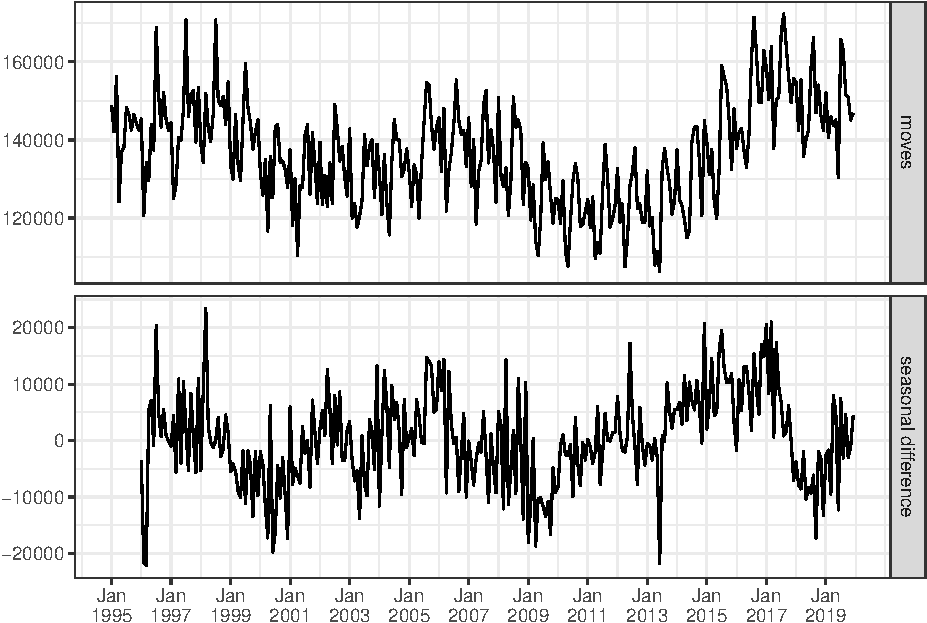
\includegraphics{../figs/freq--freq-plot-1.pdf}
\caption{\label{fig:freq-plot}Frequency of mobility (upper panel) and
seasonal differences (lower panel) and two-year moving averages (dotted
line)}
\end{figure}

The upper panel shows that there are between 11 and 7 moves per 1000
inhabitants per month. The plot suggests that the moves is cyclical with
uneven period length. We see clearly from the plot that the time series
is non-stationary and a Dickey Fuller test confirms this. The financial
crisis, which hit the Dutch housing market hard, can be seen in the dip
from 2008 onwards, with the recovery from the crisis set in during the
year of 2014. The dotted line, which in this panel can be interpreted as
the trend-cycle, illustrates clearly the connection between mobility and
the macroeconomy: the dip from 2008 onwards and the recovery from 2014
follows the financial crisis which hit both labour and housing markets
in the same periods.

From the middle panel, which shows the seasonal differences, we see that
the year on year changes are negative from January 2009 with a recovery
in 2012 and a new dip in 2013 before a real recovery from 2014.
Interestingly the lower-panel figure reveals that the year on year
changes become negative from medio 2017. This is also reported by
Statistics
Netherlands:\footnote{\url{https://www.cbs.nl/nl-nl/nieuws/2018/26/minder-mensen-verhuisd-in-eerste-kwartaal-2018}}
in 2018 there were 5 \% fewer moves than in 2017, with the decline
concentrated primarily among people younger than 50 years old. This
reflects thus an end of an increasing trend from 2014 onwards. This
shows that our suspicions of a peak in mobility frequency at the end of
2016 were not far off the mark. As suggested by the lower panel, the
monthly differences of the moves approximates a random walk. The visual
inspection of this figure reveals a fairly unpredictable long-term
pattern, with jumps hovering around zero. The moving averages suggest
indeed that the medium-term average monthly change of the series is
zero.

Summing up, the decomposition of the time series suggests that there is
no linear trend, rather a cycle with peaks roughly every 10 years. There
are furthermore strong seasonal effects with variations between the
years, meaning the seasonality contains noise. Furthermore, the
seasonality and the trend-cycle lead to autocorrelation. The next
section shows how these elements are adressed in the state space model.

\section{Model description}\label{model-description}

The ``state'' is state space models is an unobserved dynamic process
\(\theta_{t}\) for which only a noisy measurement \(y_{t}\) can be
observered. State space models are modular in the sense that the state
vector \(\theta_{t}\) is constructed by adding components deemed
necessary to characterise the time series. As mentioned in the
Introduction, DLMs are a special case of state space models with
Gaussian and independent errors. Forecasting and inference is carried
out with the recursive Kalman filter algorithm (Kalman and others 1960).
Residuals are calculated by comparing the one-step ahead predictions
from the Kalman filter with the observed values. There are many ways of
describing state space models; the model is implemented in \emph{R}
using the \emph{dlm} package, therefore the description in this section
follows the notation used in Petris, Petrone, and Campagnoli (2009).

Let \(y_{t}\) denote the logarithm of the moves in month \(t\), where
\(y_{t}\) are the observed values of underlying (unobserved) vector of
states \(\theta_{t}\). \(y_{t}\) are conditionally independent given the
state \(\theta_{t}\). The state represents a latent Markov process,
meaning that the probability of moving to the next state depends only on
the previous state. We can write this DLM as:

\[
\begin{aligned}
& y_{t} = F \theta_{t} + v_{t} & v_{t} \sim N(0, V_{t}) \\
& \theta_{t} = G \theta_{t-1} + w_{t} &w_{t} \sim N(0, W_{t}) \\
& \theta_{0} \sim N(m_{0}, C_{0})
\end{aligned}
\]

The first equation is called the \emph{observation equation} and the
second the \emph{state equation}. \(v_{t}\) and \(w_{t}\) are
uncorrelated Gaussian errors, where the observation variances are
gathered in the \(m \times m\) matrix \(V_{t}\) and system variances in
the \(p \times p\) matrix \(W_{t}\). \(F\) and \(G\) are known system
matrices of dimension \(p \times m\) and \(p \times p\) respectively.
The initial \(\theta_{0}\) are normally distributed with means \(m_{0}\)
and variances \(C_{0}\).

As mentioned, elements of the state vector \(\theta_{t}\) should be
chosen such that they reflect the characteristics of the time series in
question. The first thing we noted in the previous section was that the
time series was clearly non-stationary with no global trend. However, we
saw that periods of growth were followed by periods of decline, meaning
there were piecewise or local trends. One model that can capture such
patterns is the linear growth or local linear trend model, where the
\(y_{t}\) are noisy observations of a level \(\mu_{t}\) which varies
over time with slope \(\beta_{t}\). The dynamics of the slope itself is
modelled as a random walk. We can write the local linear trend model as
follows:

\[
\begin{aligned}
& y_{t} = \mu_{t} + v_{t} & v_{t} \sim N(0, \sigma_{v}^{2}) \\
& \mu_{t} = \mu_{t-1} + \beta_{t-1} + w_{t,1} &w_{t,1} \sim N(0, \sigma_{\mu}^{2}) \\
& \beta_{t} = \beta_{t-1} + w_{t,2} &w_{t,2} \sim N(0, \sigma_{\beta}^{2}) \\
\end{aligned}
\]

Follow the notation in Petris, Petrone, and Campagnoli (2009), we can
write the local linear trend model as:

\[
\theta_{t} = \begin{bmatrix} \mu_t \\ \beta_{t} \end{bmatrix} \quad 
G_{t} = \begin{bmatrix} 1 & 1 \\ 0 & 1 \end{bmatrix} \quad 
F_{t} = \begin{bmatrix} 1 & 0 \end{bmatrix} \quad
W = \begin{bmatrix} \sigma_{\mu}^{2} & 0 \\ 0 & \sigma_{\beta}^{2} \end{bmatrix} \quad
V = \begin{bmatrix} \sigma_{v}^{2} \end{bmatrix}
\]

Seasonality is dealt with by including a trigonometric seasonal
components to the model with a fixed periodicity of 12 months. One big
advantage with the trigonometric specification, relative to simpler
seasonal dummies, is that we allow autocorrelation to last through more
lags, resulting in a smoother seasonal pattern. This way we filter out
some of the noise seen in the figures in the previous section. By
including non-zero variances the seasonal pattern is allowed to change
trough time. Seasonality is incorporated in the DLM model by extending
the state equation with an underlying periodic process \(g_{t}\),
defined as the sum of \(j\) harmonics. For the \(j\)th harmonic, we can
write the evolution of the seasonal effects as:

\[
\begin{aligned}
&S_{j, t+1} = S_{j, t} \cos \omega_{j} + S_{j, t}^{*} \sin \omega_{j} \\ 
&S_{j, t+1}^{*} = - S_{j, t} \sin \omega_{j} + S_{j, t}^{*} \cos \omega_{j} \\
\end{aligned}
\]

with \(\omega_{j} = \frac{2 \pi t j}{s}\). We include two harmonics,
meaning that the trigonometric specification can be written on
matrix-form as:

\[
\theta_{t} = \begin{bmatrix} S_{1, t} \\ S_{1, t}^{*} \\ S_{2, t} \\ S_{2, t}^{*} \end{bmatrix} \quad
G = \begin{bmatrix} \cos \omega_{1} & \sin \omega_{1} & 0 & 0 \\ -\sin \omega_{1} & \cos \omega_{1} & 0 & 0 \\ 0 & 0 & \cos \omega_{2} & \sin \omega_{2} \\ 0 & 0 & -\sin \omega_{2} & \cos \omega_{2} \\ \end{bmatrix} \quad
F = \begin{bmatrix} 1 & 0 & 1 & 0\end{bmatrix} \\ \quad
W = \begin{bmatrix} \sigma_{S_{1}}^{2} & 0 & 0 & 0 \\ 0 & \sigma_{S_{1}^{*}}^{2} & 0 & 0 \\ 0 & 0 & \sigma_{S_{2}}^{2} & 0  \\ 0 & 0 & 0 & \sigma_{S_{2}^{*}}^{2} \end{bmatrix}
\]

The two components discussed so far (trend and seasonal) remove much of
the autocorrelation, however a Ljung-Box test confirmed that the
residuals of a model consisting of only were still not white noise. One
way of dealing with the residual autocorrelation is to include
autoregressive elements into the state space model. On the basis of the
partical autocorrelation function show in Appendix A, and further
analysis with an AR(2) model we choose a to include an AR(4) with two
higher order lags - namely lags 7 and 12. Consequently, the
autoregressive component of our state space model is an AR(4) model with
`gaps'. This can be cast in state space form using the following trick:

\[
\begin{bmatrix}
\mu_{1,t} \\ \mu_{2,t} \\ \mu_{7,t} \\ \mu_{12,t} 
\end{bmatrix} =  \begin{bmatrix} 
\phi_{1} & 1 & 0 & 0 \\ 
\phi_{2} & 0 & 1 & 0 \\
\phi_{7} & 0 & 0 & 1 \\
\phi_{12} & 0 & 0 & 0 
\end{bmatrix} \begin{bmatrix} 
\mu_{1,t-1} \\ \mu_{2,t-1} \\ \mu_{7,t-1} \\ \mu_{12,t-1} 
\end{bmatrix} \begin{bmatrix}
u_{t} \\ 0 \\ 0 \\ 0 
\end{bmatrix}
\]

which gives

\[
\mu_{1,t} = \phi_{1} \mu_{1,t-1} + \phi_{2} \mu_{1,t-2} + \phi_{7} \mu_{1,t-7} + \phi_{12} \mu_{1,t-12} + u_{t} \quad u \sim N(0, \sigma^{2}_{u})
\]

Notice that the standard routine for creating autoregressive elements in
the \emph{dlm} package do not allow for `gaps' in the included lags. In
order to estimate such a model we need to implement system matrices of
an AR(12) where the parameter of lags not included in the model are set
to zero:

\[
G = \begin{bmatrix} 
\phi_{1}  & 1      & 0      & 0      & \cdots & 0      & \cdots & 0      \\
\phi_{2}  & 0      & 1      & 0      & \cdots & 0      & \cdots & 0      \\
0         & 0      & 0      & 1      & \cdots & 0      & \cdots & 0      \\
\vdots    & \vdots & \vdots & \vdots & \ddots & \vdots & \ddots & \vdots \\
\phi_{7}  & 0      & 0      & 0      & \cdots & 1      & \cdots & 0      \\
\vdots    & \vdots & \vdots & \vdots & \ddots & \vdots & \ddots & \vdots \\
0         & 0      & 0      & 0      & \cdots & 0      & \cdots & 1      \\
\phi_{12} & 0      & 0      & 0      & \cdots & 0      & \cdots & 0
\end{bmatrix} \quad F = \begin{bmatrix} 1 & 0 \cdots \end{bmatrix} \quad W = diag(\sigma_{u}^{2}, 0, ...)
\]

The resulting composite model (trend, seasonal and autoregressive) has a
state vector \(\theta_t\) of length 7:
\(\theta_t = (\mu_t, \beta_t, S_{1, t}, S_{1, t}^{*}, S_{2, t}, S_{2,t}^{*}, \mu_{1,t})'\).
In order to apply the Kalman filter we first need to determine the
unknown model parameters. Unknown parameter are the variances of the
error terms, in effect hyper-parameters, and the parameters for the
autoregressive terms. We chose to estimate all of them using maximum
likelihood (see Petris, Petrone, and Campagnoli 2009, ch.~4). As we have
seen, the matrix \(W\) contains 9 potentially non-zero parameters:
\(\sigma_{v}^{2}\), \(\sigma_{\mu}^{2}\), \(\sigma_{S_{2}}^{2}\),
\(\sigma^{2}_{u}\), \(\phi_{1}\), \(\phi_{2}\), \(\phi_{7}\), and
\(\phi_{12}\). Note that the parameters governing the autoregressive
component are estimated subject to stationarity restrictions (Monahan
1984).

\section{Results}\label{results}

\subsection{Estimated parameters}\label{estimated-parameters}

As we saw in the previous section, the trend component contains two
error terms with their own variances - one for the level and one for the
slope. Initial runs with the model discussed so far revealed that two
special cases fit the data better than the general formulation. The
first special case is obtained by setting \(\sigma^{2}_{\mu} = 0\),
sometimes referred to as the integrated random walk or the smooth trend
model (REF). In this specification, all noise is captured by the slope,
meaning that the local linear trend becomes rather smooth (hence the
name). In the rest of the paper will refer to this model as DLM1. A
second special case is a model in which \(\sigma^{2}_{\beta} = 0\),
where all stochasticity is removed from the dynamics of the slope. In
this formulation the estimated \(\beta_{t}\) reflect the long run growth
of the time series rather than the local growth. As we saw in Figure
\ref{fig:freq-plot}, the slope representing long-run growth (moving
averages of the monthly differences) is almost completely flat. However,
due to the inclusion of the autoregressive elements the forecasted
values can diverge from the long-term growth in the short-run. More
specifically, a one-step-ahead forecast \(\hat{y}_{t + 1}\) reflects up
to 12 lagged values of the time series \(y_{t}\). If the time series
diverges from the long-run growth in this interval, this will also be
picked up by the forecasts. We will refer to this model as DLM2.

The estimated parameters are shown in Table
\ref{tab:estimated-parameters}. We see that the observation variance
\(\sigma_{v}^{2}\) is very close to zero, indicating a high level of
precision of the observations. The estimated parameters of the
autoregressive parts are very similar between the two models, except for
the parameter of the second lag which takes positive values for DLM1 and
negative values for DLM2.

\begin{table}[t]

\caption{\label{tab:estimated-parameters}Estimated variances and AR parameters}
\centering
\begin{tabular}{lllll}
\toprule
Parameter & DLM1 &   & DlM2 &  \\
\midrule
 & Estimate & SE & Estimate & SE\\
$\sigma_{v}^{2}$ & 1.523e-08 & 5.047e-07 & 1.523e-08 & NaN\\
$\sigma_{\mu}^{2}$ & 0 & 0 & 0.0001427 & 3.319e-05\\
$\sigma_{\beta}^{2}$ & 2.471e-06 & 1.024e-06 & 0 & 0\\
$\sigma_{S_{2}}^{2}$ & 7.618e-06 & 4.098e-06 & 7.602e-06 & 3.808e-06\\
\addlinespace
$\sigma^{2}_{u}$ & 0.001287 & 0.0001348 & 0.001031 & 0.0001258\\
$\phi_{1}$ & -0.637 & 0.2356 & -0.6904 & 0.2311\\
$\phi_{2}$ & 0.03081 & 0.1221 & -0.05365 & 0.1274\\
$\phi_{7}$ & -0.4415 & 0.09384 & -0.4879 & 0.09533\\
$\phi_{12}$ & 0.4486 & 0.06234 & 0.4349 & 0.06164\\
\bottomrule
\end{tabular}
\end{table}

\subsection{Filtering and smoothing estimates of the
moves}\label{filtering-and-smoothing-estimates-of-the-moves}

With estimates of the unknown parameters we use the Kalman filter to
obtain the filtered distribution of \(\theta_{t}\) conditional on the
observed series up to \emph{t}, \(\theta_{t} | y_{1}, y_{2},...,y_{t}\).
Forecasts of the next observation \(y_{t+1}\) based on observations up
to \(t\), are produced by first computing the state vector
\(\theta_{t+1}\) and then predicting \(Y_{t+1}\). Similarly, an n-step
ahead forecast \(Y_{t+n}\) is based on calculation of the n-step ahead
state vector \(\theta_{t+n}\). We can write the forecast function as
\(f_{t} = E(Y_{t+n} | y_{1}, y_{2}, ....y_{t})\). In addition we
estimate a smoothing distribution of the components, representing the
past values of the states given all observed values
\(\theta_{t} | y_{1}, y_{2},...,y_{s}\) where \(s \ge t\).

The one-step ahead predictions from the Kalman filter, or filtered
values, from both of the models are displayed in Figure
\ref{fig:dlm-filtered}, together with Root Mean Square Error (RMSE)
calculated on basis of the residuals (one-step-ahead forecast errors).
The adaptive nature of the Kalman algorithm causes the filtered values
in the first periods to veer quite far off the observed values (not
shown in the figure). We therefore discard the three first years when
calculating the RMSE. It is clear from the figure that DLM2 fits the
data somewhat better than the DLM1 model, though the difference is not
dramatic. A residual check showed that the normality assumption of
dynamic linear models is justified for these models (see Appendix B for
a residual plot of DLM2).

\begin{figure}
\centering
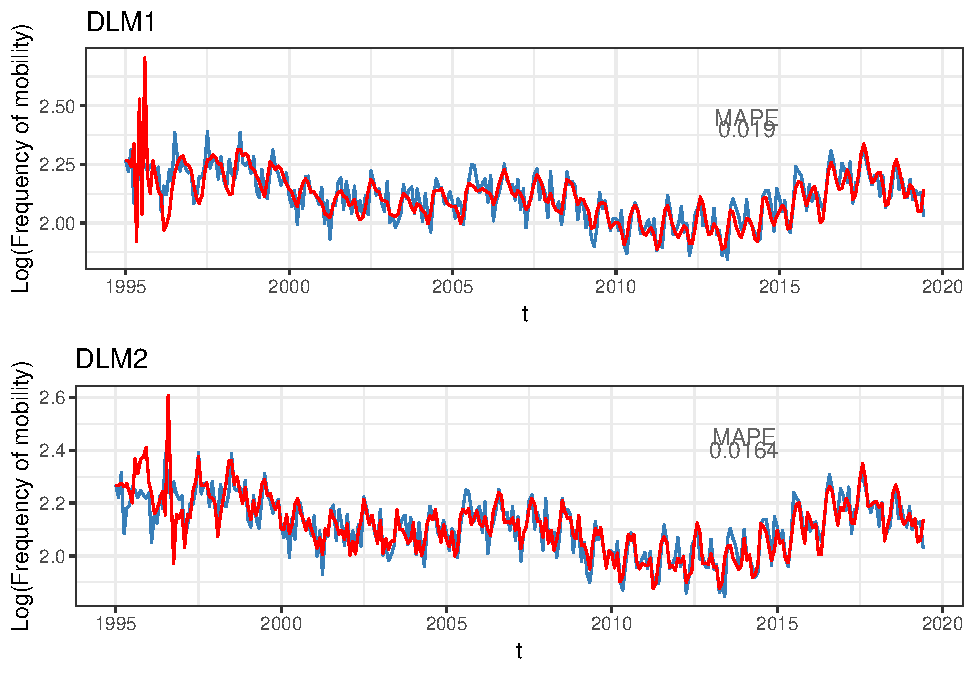
\includegraphics{../figs/freq--dlm-filtered-1.pdf}
\caption{\label{fig:dlm-filtered}One-step-ahead predictions (solid line),
observed data (dotted line) and RMSE (calculated from January 1998)}
\end{figure}

Figure \ref{fig:ci-comparison} shows the one-step ahead predictions
along with the 95 percent prediction intervals of DLM1 and DLM2 for the
months between January 2010 and December 2018. The interval is
calculated using the standard deviation of the filtered values (Petris,
Petrone, and Campagnoli 2009, ch.~3). From this plot we clearly see that
DLM1 systematically predicts a higher moves than DLM2 from 2014 to about
2017. Athough barely visible in the figure, the prediction interval of
DLM1 is slightly smaller than that of DLM2.

\begin{figure}
\centering
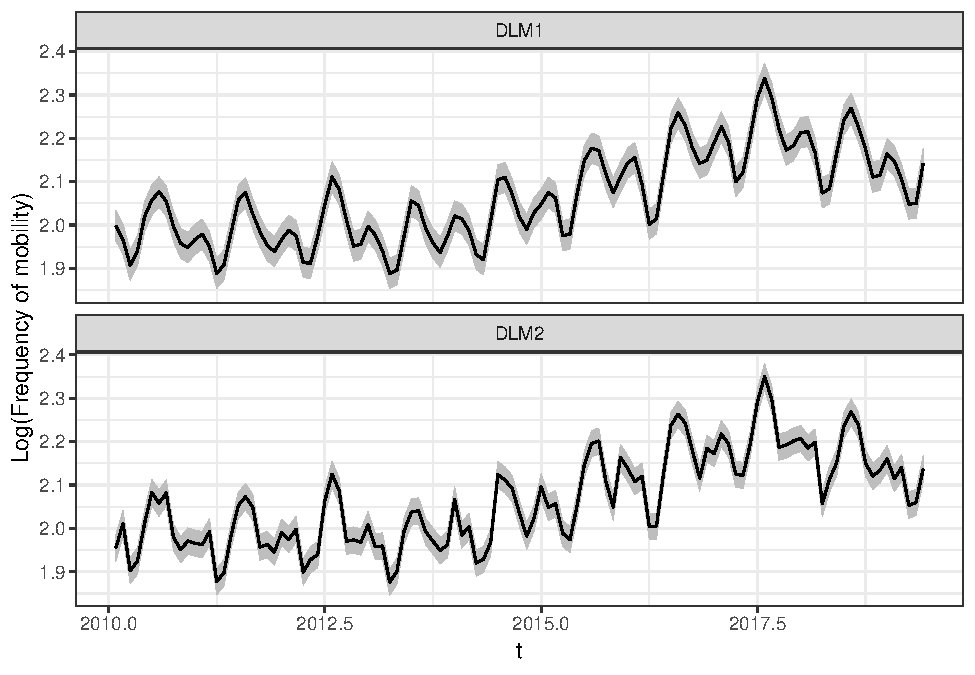
\includegraphics{../figs/freq--ci-comparison-1.pdf}
\caption{\label{fig:ci-comparison}Filtering estimate and 95 percent
prediction intervals}
\end{figure}

The smoothing estimates for the trend-cycle component and for the
seasonal effects are shown in Figure \ref{fig:dlm-smoothed}. From the
left panels we can pin-point the recent peak in the trend-cycle to March
2017. We see a visible difference between DLM1 and DLM2, where the
former model produces a much smoother The right panels show how the
seasonal effects vary over time; at the start of the time series the
within-year cycle exhibites one pronounced maximum (July) and one
minimum (March). However, from around the middle of the series, there is
gradually another local maximum within each year (Janauary). This means
that the seasonal patterns in the model captures well the development of
the seasonal factors from the raw data.

\begin{figure}
\centering
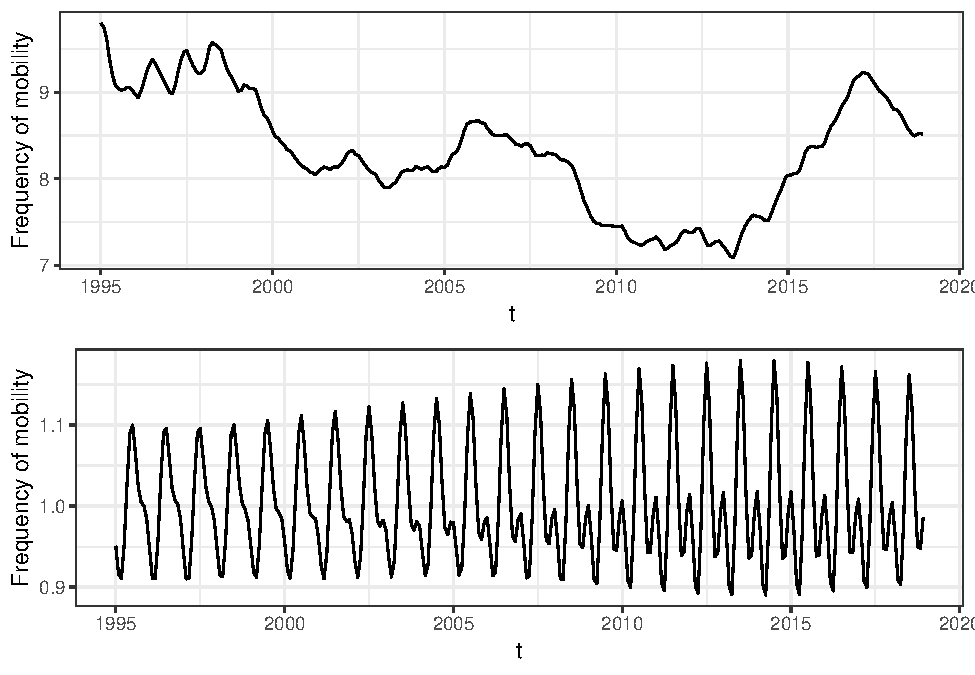
\includegraphics{../figs/freq--dlm-smoothed-1.pdf}
\caption{\label{fig:dlm-smoothed}Smoothing estimate of the trend-cycle and
seasonality}
\end{figure}

\section{Discussion}\label{discussion}

\subsection{Cross validation: evaluation over a rolling
origin}\label{cross-validation-evaluation-over-a-rolling-origin}

In this section we evaluated the forecasting accuracy of the models
described in the previous sections. Our primary interests here are how
well the models predict data points that have not been used for
estimation (out-of-sample), and how performance varies with the length
of the forecast horizon, whereby accuracy measures are calculated for
several forecast lengths (in effect N-step forecast). For
cross-sectional data such evaluations are commonly carried out by
estimating the model on a training data set and evaluating it on an
independent test data set. In order to control for effects arising from
the composition of the training data, it is common to repeat this
procedure with different training and test data sets using k-fold cross
validation. Due to the serial autocorrelation and potential
non-stationarity in the data, it is common to choose a test set that
does not contain observations occuring prior to the observations in the
training data (Bergmeir and Benítez 2012). Recent literature suggests
that standard cross-validation can be applied to certain time series
models (Bergmeir, Hyndman, and Koo 2018), however, due the Markovian
structure of the Kalman filtering algorithm, we suspect that the
technique would not work for the state space models discussed in the
previous section. Therefore we follow the conventional approach for
evaluating time series accuracy; namely evaluation over a
\textit{rolling forecasting origin} (Tashman 2000), where we succesively
extend the training data and produce forecasts of the test data. The
last point of the training data in each iteration is referred to as the
\textit{origin} \(T\), since the origin on which the forecast is based
rolls forward in time. In this approach, the training data consists of
observations between \(t = 1, ..., T\) and forecasts are generated for
time periods \(T+1\), \(T+2\), \ldots{}, \(T+N\). This procedure is
illustrated in Figure \ref{fig:rolling-forecast-example}. The movement
along the x-axis shows how the origins (vertical dotted line) ``roll''
forward in time, where the model is estimated on the training data
(black solid line). The model perfomance is then evaluated by averaging
the prediction errors over different forecast horizon (dotted horizontal
lines).

\begin{figure}
\centering
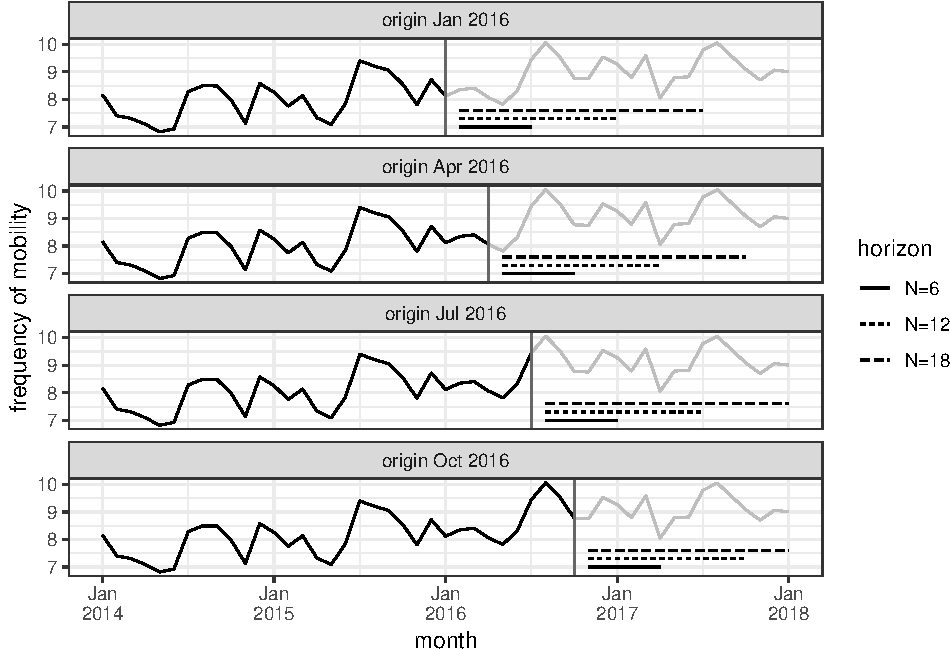
\includegraphics{../figs/freq--rolling-forecast-example-1.pdf}
\caption{\label{fig:rolling-forecast-example}Illustration of rolling
forecasting origin: training data (solid black line), origin (vertical
dark grey line), forecast horizion (dotted horizontal lines) and test
data (grey line)}
\end{figure}

We evaluate forecasting performance on three time horizons: \(N=6\),
\(N=12\) and \(N=18\) - meaning that, for each origin, we calculate
three indicators of accuracy; one for a half year forecast, one for a
year and one for one and a half year. We are interested in assessing the
performance around the changepoint of the trend-cycle. From the previous
section we identified this as March 2017 (see Figure
\ref{fig:dlm-smoothed}). In order to evaluate the performance of the
models on both sides of the changepoint we include origins within 12
months before and after March 2017. Including the changepoint itself we
have in total 25 forecasting origins: T = March 2016, February 2016,
\ldots{}, June 2017.

In order to ensure independence between the test and training sample, we
estimate the models on the relevant training data of each origin
forecast. As such, it is possible that estimated parameter values differ
between the different origins. The resulting mean and standard
deviations, shown in Table \ref{tab:par-comparison} in the Appendix,
reveal that differences in training data has a very limited effect on
the estimated parameters. This also gives us confidence that there is
enough data for estimation even on the first origin.

The forecast performance of the DLMs is assessed by comparing
forecasting accuracy with that of three other popular models. The first
of these is a naïve seasonal model (Naïve), where the forecast of a
specific month is simply the value of the same month of the previous
year. Despite its simplicity this model is useful with data with no
clear trends. Since the model assumes no trend, we expect this model to
perform particularly well around the changepoint. The next model is the
Holt-Winters method with multiplicative seasonality (Holt 2004; Winters
1960). This model is an extention of the simple exponential smoothing
model, allowing for forecasts with a trend. Using the function
\({\tt HoltWinters()}\) in base \emph{R}, the smoothing parameters of
the model are selected automatically, for each origin, with the default
initial values. This model type performs particularly well on data with
a clear trend, and we therefore expect it to forecast accurately before
the changepoint and increasingly worse around and after it.

Furthermore, exponential smoothing can also be formulated on state space
form, allowing for a much more general models of exponential smoothing
methods. We will refer to this model type as ETS (Error, Trend,
Seasonal). An advantage of casting exponential smoothing models on the
stochastic state space form is the possibility of generating prediction
intervals - either analytically or by simulation. This furthermore
allows information criteria to be used for model selection, meaning that
all combination of trend-, seasonal and error components can be explored
(R. J. Hyndman et al. 2002). The automatic model selection is carried
out using the \({\tt ets()}\) function with default values for all
arguments, meaning that selection is based on the corrected Akaike's
Information Criterion (AICc).

Finally we include a seasonal ARIMA model into the comparison.
Identification of the model is carried out using the
\({\tt auto.arima()}\) function on the whole sample (R. J. Hyndman and
Khandakar 2008), and results in an ARIMA(2,1,5)(2,1,1). This is thus a
model with double differencing, with yearly and monthly MA(2), and
yearly AR(5) and monthly AR(2). For each origin we reestimate the model
parameters on the respective training data. We also tried the automatic
selection for each origin with only marginal differences in results.

Table \ref{tab:error-comparison} shows the overall forecast accuracy
across all origins for all models. This investigating the distribution
of accuracy accross ``folds'' (in this case forecasting origins). The
table shows both RMSE and mean absolute percentage error (MAPE),
averaged over origins, of each of forecasting horizon (6 months, 12
months, 18 months). In order to asses whether the accuracy varies
between origins the table also shows the standard deviation of RMSE and
MAPE. From the table we see that both RMSE and MAPE of the DLM2 are
quite similar across all forecast horizons, however with a slight
advantage of DLM2. Not suprisingly, accuracy deteriorates as N
increases, although not dramatically so: in the case of DLM2, the mean
RMSE for N=6 is 0.39, compared to 0.53 for N=18. The limited
deterioration in forecast accuracy is not shared with the ARIMA and
Holt-Winters models, which both see substantial increases in forecasting
errors as the forecast horizon increases. The mean RMSEs of the Naïve
model is remarkably stable across all forecast horizons, and it is, in
general, the least accurate model. We see that the ETS model outperforms
DLM2 for the shortest forecast horizon in terms of both RMSE and MAPE.
For forecasts of 12 or 18 months the ETS model performs slightly better
than DLM2 in terms of RMSE and slightly worse in terms of MAPE. Since
squared errors gives a heavier penalty to large forecast errors than
absolute errors, this means that DLM2 produces the smallest median
forecast error and ETS the smallest mean forecast error.

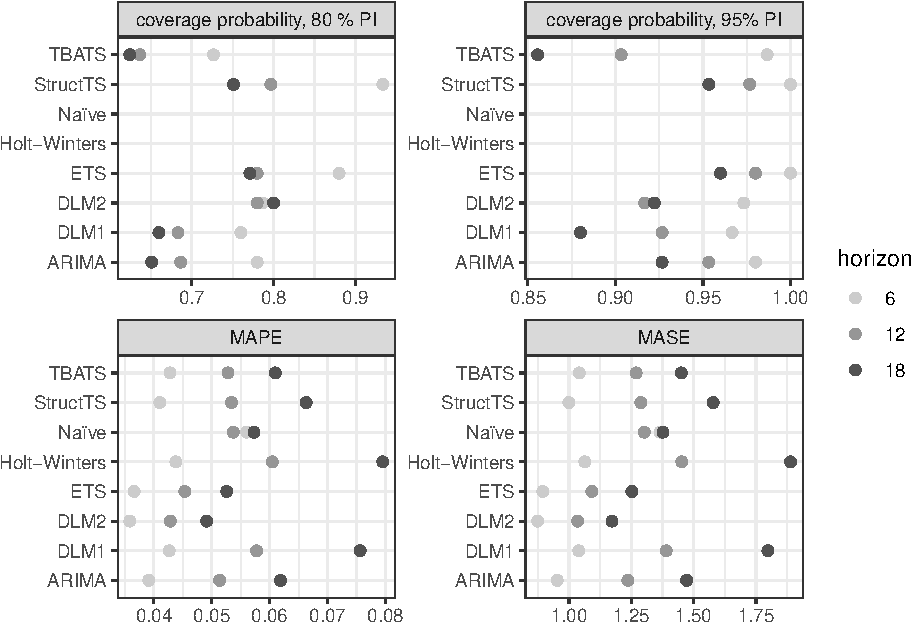
\includegraphics{../figs/freq--error-comparison-1.pdf}

Figure \ref{fig:rmse-origins} delves further the variation in
forecasting performance across origins, showing the MAPE per origin and
model for the three forecast horizons. In all forecast horizions the two
DLMs are the best performing models in the interval between December
2016 and December 2017, with the exception of origins right after March
2017 where the Naïve model perfoms best. We see that the ARIMA,
Holt-Winters and the ETS models all perform better than the DLMs on the
part of the time series where there is a clear trend in the training
data that at least partially extends into the test data (until December
2016). As Table \ref{tab:error-comparison} showed, the higher forecast
accuracy of the ETS model relative to the DLMs occurs primarily for a
short forecast horizon. The relatively high MAPE for the DLMs prior to
December 2016. Finally, the difference in performance between the two
DLMs is, in general, minimal. However, the 6 month forecasts from medio
2017 onwards differ somewhat between the models, with DLM2 performing
better than the DLM1.

\begin{figure}
\centering
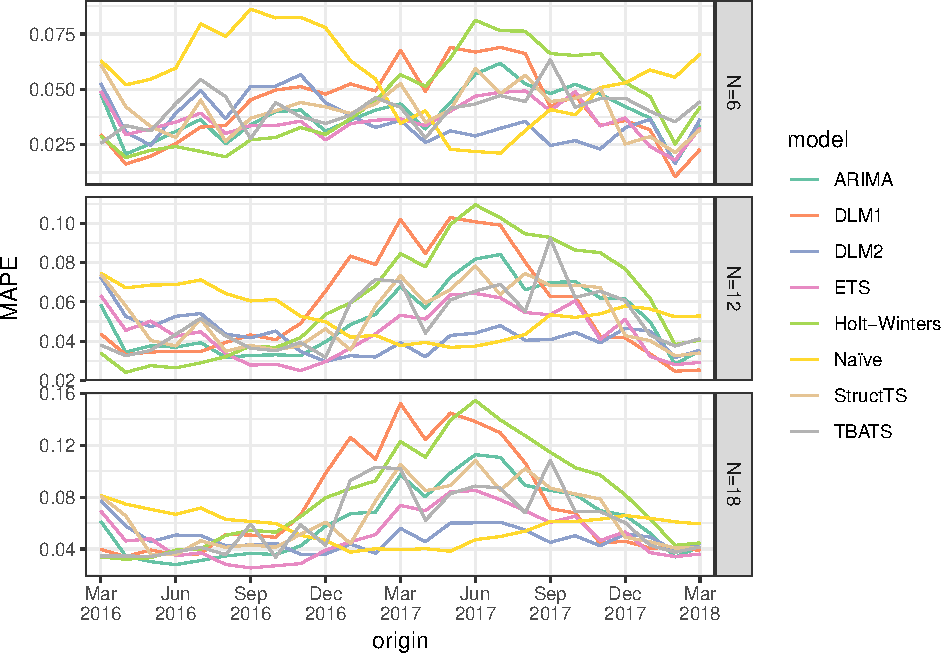
\includegraphics{../figs/freq--rmse-origins-1.pdf}
\caption{\label{fig:rmse-origins}MAPE by origin and forecast horizon}
\end{figure}

Figure \ref{fig:rmse-origins} showed how the forecasting performance
varied between origins; it suggested that the DLMs performed poorly,
relative to other models, where a trend carried over from the training
data to the test data and good relative to other models otherwise. Of
course our initial interest in this exercise was motivated by a
potential trend change. Therefore we zoom in on the forecasted values of
the moves around the changepoint. Figure \ref{fig:forecast-2017-2018}
compares the forecasts of all models in the period January 2017 to
December 2018. The grey dots represent forecast from different origins,
the solid line represents the average value of the forecasts across all
origins and the dotted line is the data. The figure shows clearly the
divergence in forecasting performance between the DLMs and the ARIMA and
Holt-Winters models. The Holt-Winters model systematically overpredicts
the migration frequency already from June 2017, meaning that the
forecasted frequency exceeds the data for all origins. For the ARIMA
model this occurs from October 2017. In the case of the DLMs the last
forecasted point with a value lower than that of the data occurs in May
2018.

\begin{figure}
\centering
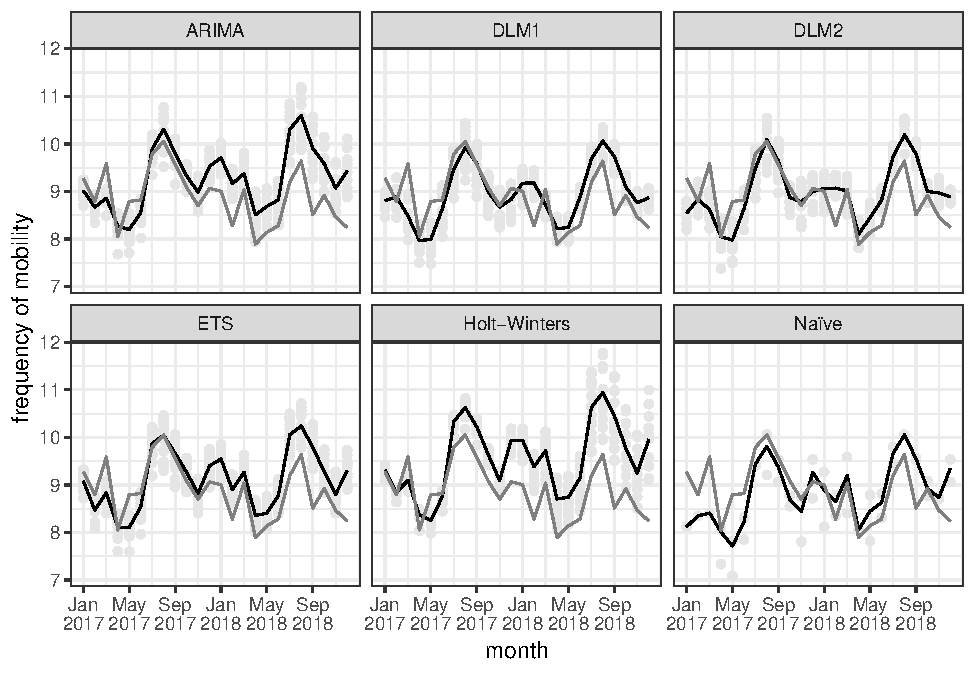
\includegraphics{../figs/freq--forecast-2017-2018-1.pdf}
\caption{\label{fig:forecast-2017-2018}Forecasted (light grey dots),
forecast averaged over origins (black line) and observed (dark grey
line) moves}
\end{figure}

\subsection{Forecasting migration frequency from January 2017
onwards}\label{forecasting-migration-frequency-from-january-2017-onwards}

As mentioned in the Introduction, the realisation that 2017 possibly
represented a turning point in the cycle of the moves triggered our
initial interest in developing the state space model. Then it is
relevant to ask what the second state space model tell us about the
development of the frequency of migration from 2017 onwards. In our case
we were particularly interested in the development of the yearly
frequency the coming couple of years. Figure \ref{fig:forecast-2017}
shows a two-year forecast of both the monthly and yearly moves with
their 95 percent prediction intervals, where the last period of the
training data is December 2016. For simplicity, the yearly frequency is
calculated by aggregating the monthly frequencies within that year. As a
comparison, we also show results the same forecast using the ETS model
discussed in the previous section. The automatic selection procedure
results in an ETS(M, Ad, A): a model with multiplicative errors, damped
additive trend and additive seasonal effects.

\begin{figure}
\centering
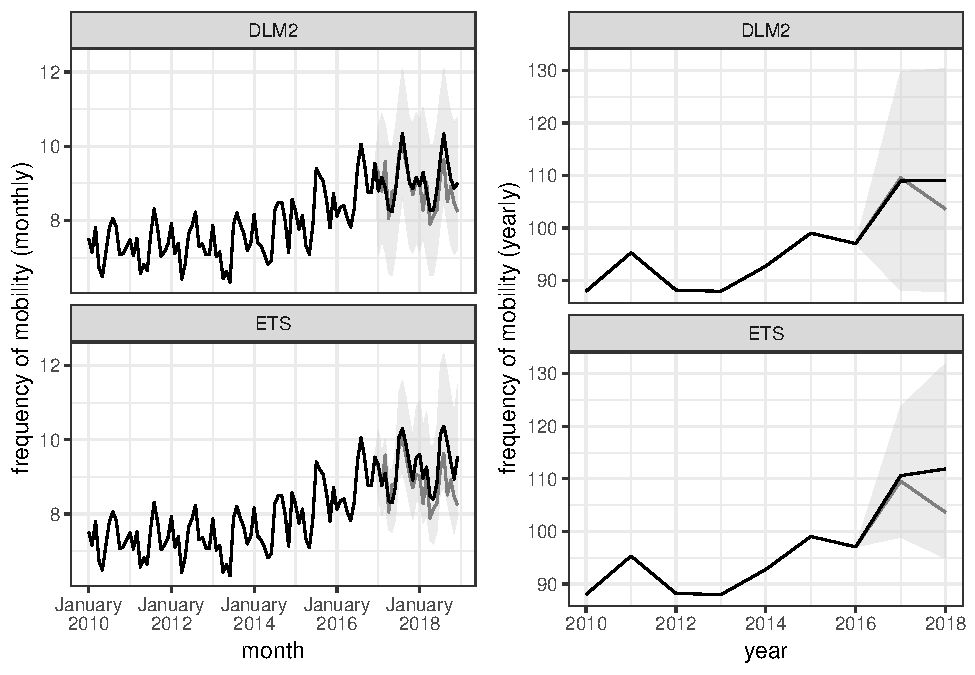
\includegraphics{../figs/freq--forecast-2017-1.pdf}
\caption{\label{fig:forecast-2017}Two-year forecast (black line) of monthly
(left) and yearly (right) moves and test data (dark grey line) and 95
percent prediction interval}
\end{figure}

\begin{figure}
\centering
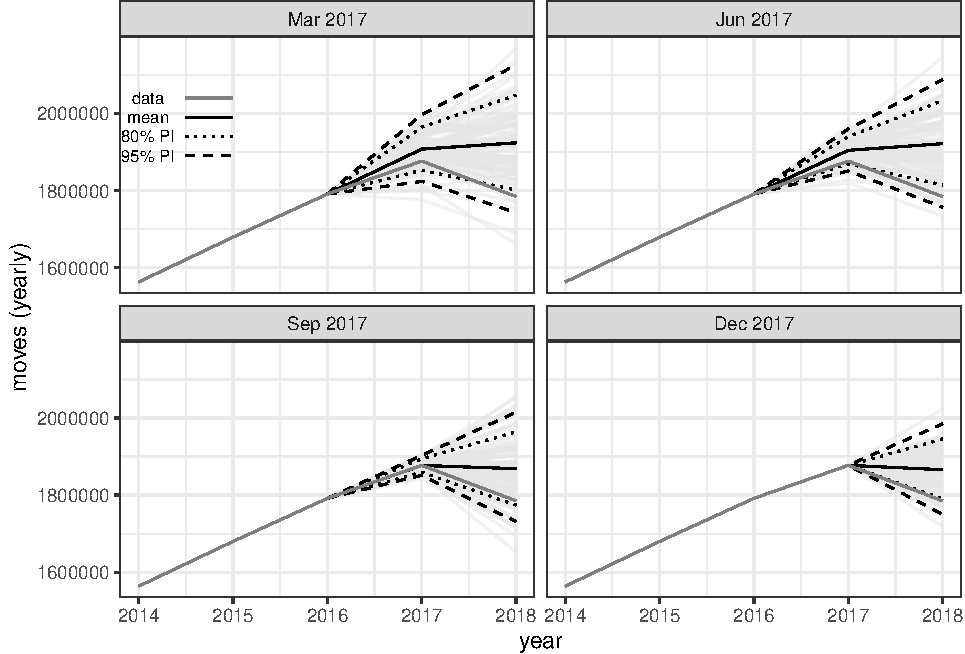
\includegraphics{../figs/freq--mc-intervals-dlm-1.pdf}
\caption{\label{fig:mc-intervals-dlm}Monte Carlo simulations of prediction
intervals, DLM2}
\end{figure}

\begin{figure}
\centering
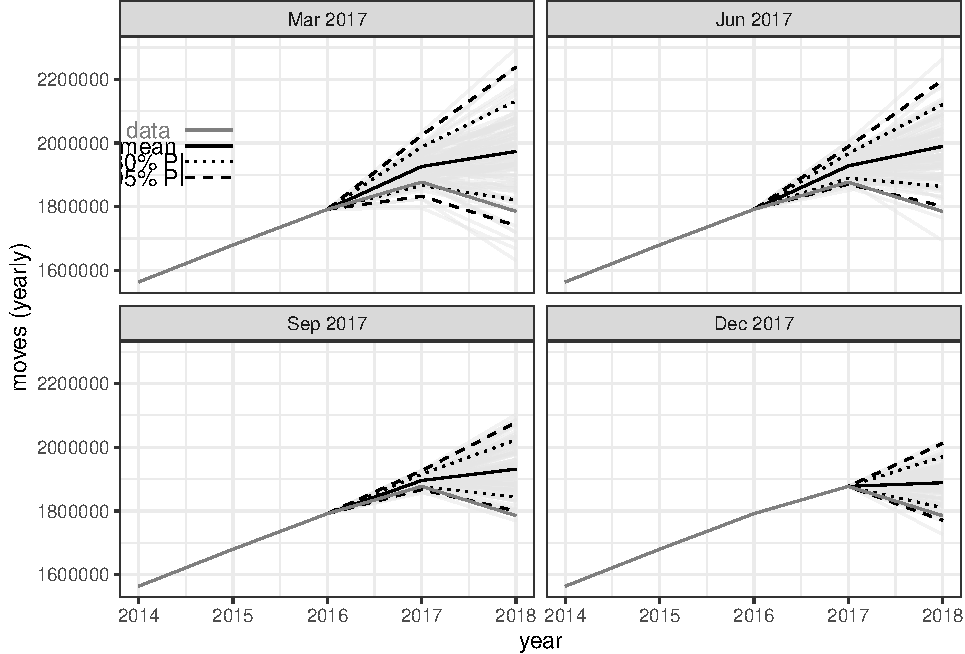
\includegraphics{../figs/freq--mc-intervals-ets-1.pdf}
\caption{\label{fig:mc-intervals-ets}Monte Carlo simulations of prediction
intervals, ETS}
\end{figure}

At first glance, the point forecast of the monthly frequency (left part
of the figure) is quite similar across models, although the prediction
interval of ETS is smaller. Both models forecast 2017 accurately, and
they both systematically overestimate the test data in 2018. As the
right left panels of Figure \ref{fig:forecast-2017} shows, the yearly
moves actually declines between 2017 and 2018, and none of the models
were able to capture this sudden decline. However, we see ETS is much
more ``positive'' about (i.e., overestimates more substantially) the
yearly frequency than DLM2. As we discussed earlier, both of these
models can allow a short-run forecasts to diverge from a long-run trend
growth. The figure thus suggests that the models produce quite similar
short-run forecasts, but they differ in terms of their expected long-run
growth. As a side note, the Naïve model would in fact predict the yearly
frequency of 2018 very well. But a clock without battery also shows the
right time twice a day.

\section{Conclusion}\label{conclusion}

In this paper we have developed a state space model for short-to medium
term univariate forecast of monthly moves in the Netherlands. The moves
is defined as the number of internally migrated persons countrywide
(within- and between-municipality) per month divided by the population.
This is an important input into the cohort-component model used for our
regional population projections; the need for this modelling exercise
arose as we suspected that the end of our yearly series represented the
top of a cycle.

The results presented in the previous section show that the state space
model (DLM) quite accurately forecasts both monthly and yearly moves
until end 2018, based on data up to end 2016. In particular, the model
would have given us a very accurate picture of the development of the
moves until end of 2017. More generally, the model performed comparably
or even better than a number of popular univariate forecasting in a time
interval between end of 2016 to end of 2017. One of the most remarkable
feature about the forecasts of the DLM was the relatively limited
deterioration in forecast accuracy as the forecast horizon increased.

The most important reason was that the local linear growth component
ensured a certain ``conservatism'' for forecast horizons above 12
months. The high signal-to-noise rate implied that the estimated local
growth rate evolved slowly over time. The only other model mimicking
this behaviour was the ETS model - itself also a state space model. An
easy critique of this result is that a model that predicts that `what
goes up must eventually come down' is of limited value. Yet such
criticism misses the point that the local linear growth component in
effect incorporates not only local, but to some extent global,
characteristics of the time series. As such, this model also answers the
question ``come down to what?''.

Although the focus of this paper was univariate forecasts, one of the
biggest advantages of the structural model developed in this paper,
relative to automatically selected models such as ETS, is the easy with
which covariates can be included. Future research should focus on
investigating whether model performance can be improved by including
covariates for which there are reliable short- to medium-term forecasts
- for example unemployment levels. Splitting up the time series into
several age groups (dynamic hierarchical models) will probably make such
an exercise easier, and is probably a fruitful venue for future
research. A more theory-driven model with covariates could also provide
extra information about the merits of the simpler univariate approach
presented.

\section{Appendix A}\label{appendix-a}

In addition to the cycle, there are strong seasonal patterns that seem
to vary over time. The seasonal subseries plot in Figure
\ref{fig:freq-month-plot} shows the movement per year and average per
month (lower panel), and the horizontal lines in the figure indicating
the means for each month. This plot enables us to see the underlying
seasonal pattern clearly, and it also shows the changes in seasonality
over time. The figure shows that the highest frequency is, on average,
in August and July while the lowest is in April. We also see there is
quite some variation between the years: the differences between the
months were more pronounced in the early part of the time series than in
later years. The lower panel suggests a sinusoidal pattern with two
peaks within one year - one peak in the summer and one at the end of the
year.

Finally, we check whether there is a linear relationship between lagged
variables of the time series (autocorrelation). Figure
\ref{fig:autocorr-plot} reveals a large and positive autocorrelation for
small lags, since observations nearby in time tend to be similar in
size. We also see that strong autocorrelation in lags that are multiples
of the seasonal frequency (12, 24, and 36), which is due to the
seasonality discussed above. The slow decline is related to the
trend-cycle while the `scalloped' pattern is related to the seasonality.
In terms of lag selection for an ARIMA model, the significant spikes at
the first and second lag in the partial autocorrelation plot in the
lower figure suggests that we should include at least two autoregressive
terms (R. J. Hyndman and Athanasopoulos 2018).

\begin{figure}
\centering
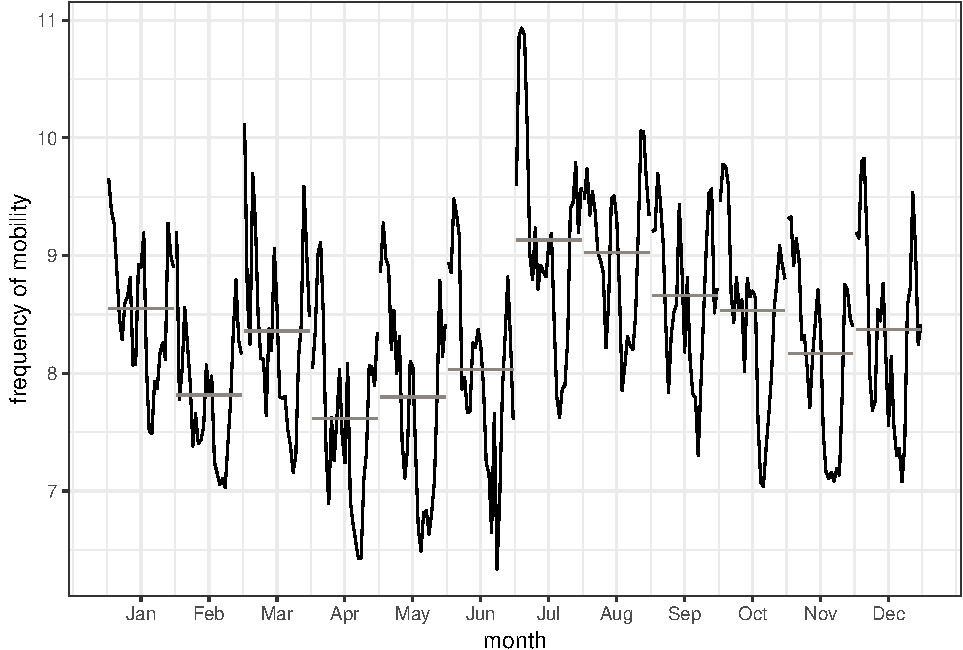
\includegraphics{../figs/freq--freq-month-plot-1.pdf}
\caption{\label{fig:freq-month-plot}Seasonal subseries plot of the moves}
\end{figure}

\begin{figure}
\centering
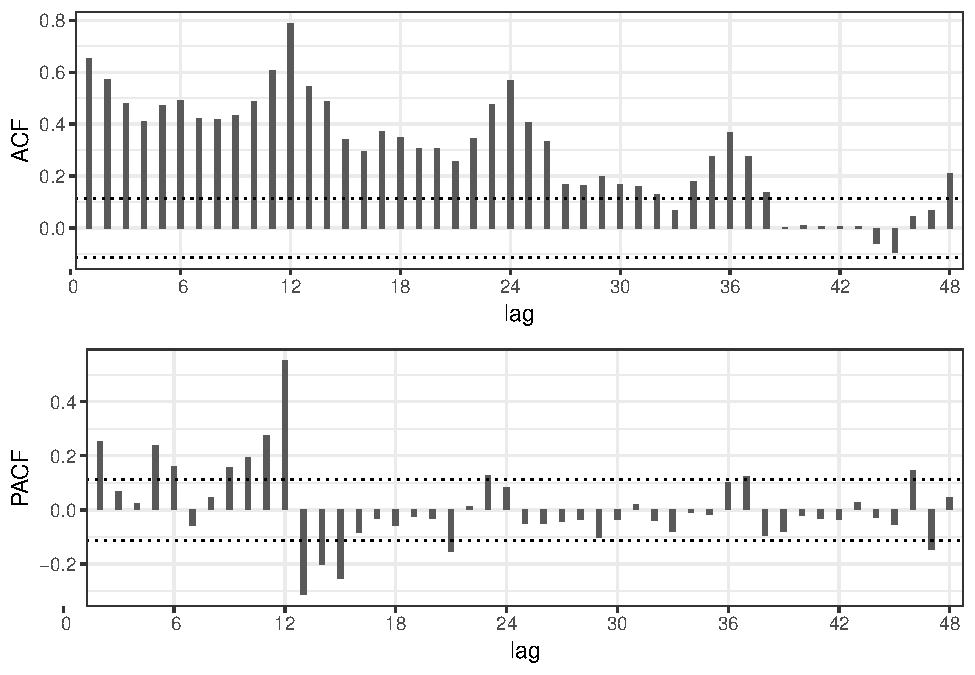
\includegraphics{../figs/freq--autocorr-plot-1.pdf}
\caption{\label{fig:autocorr-plot}Autocorrelation function of the moves}
\end{figure}

\section{Appendix B}\label{appendix-b}

\begin{figure}
\centering
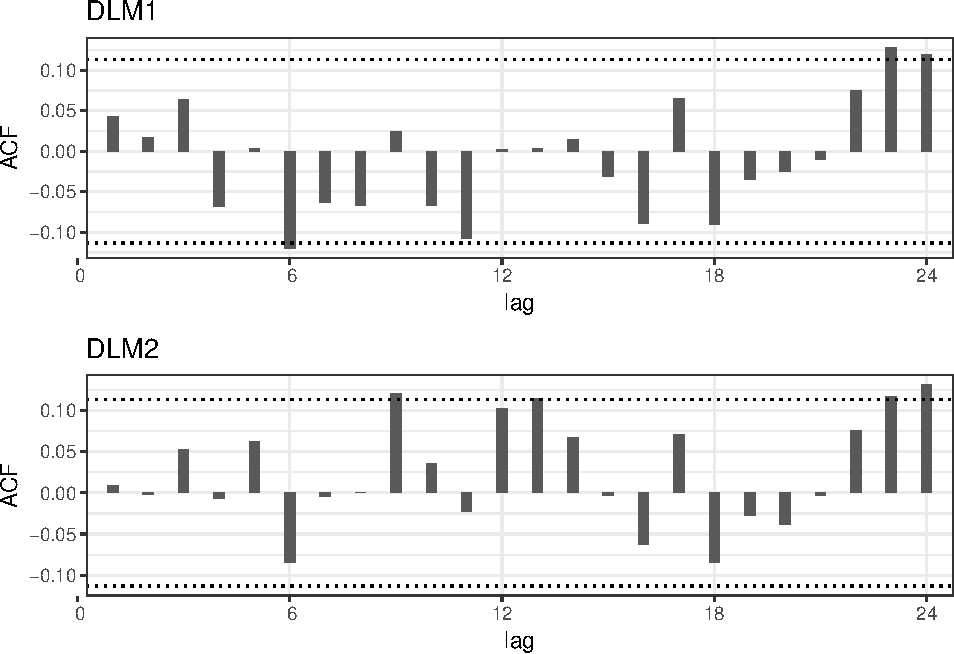
\includegraphics{../figs/freq--residual-autocorr-1.pdf}
\caption{\label{fig:residual-autocorr}Autocorrelation function of the
standardised residuals}
\end{figure}

\begin{figure}
\centering
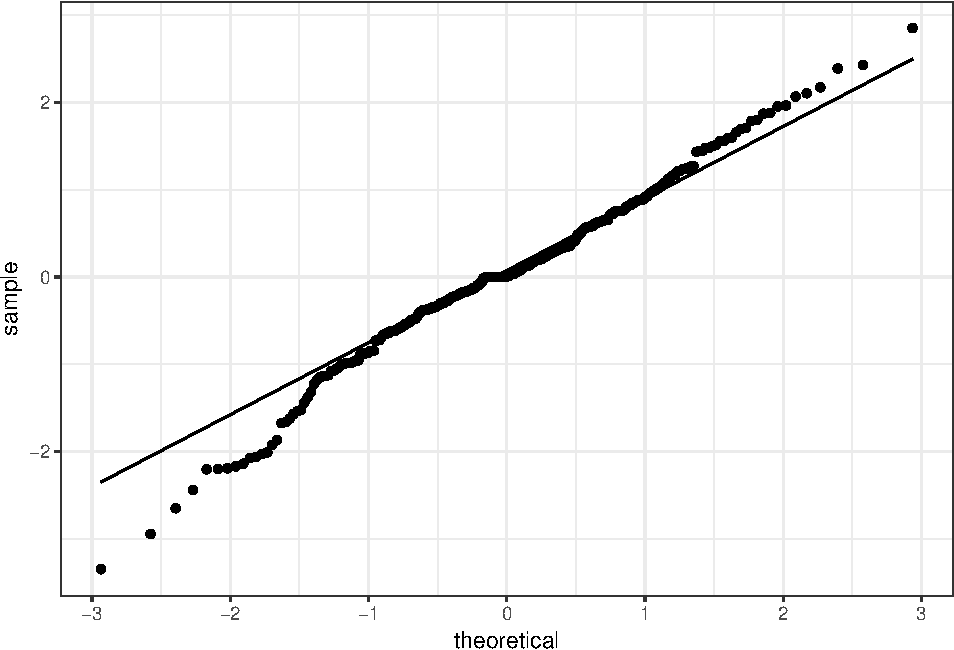
\includegraphics{../figs/freq--qqnorm-1.pdf}
\caption{\label{fig:qqnorm}Normal probability plot of standardized
one-step-ahead forecast errors of DLM2}
\end{figure}

\begin{table}[t]

\caption{\label{tab:par-comparison}Mean and standard deviation of the estimated parameters}
\centering
\begin{tabular}{lllll}
\toprule
Parameter & DLM1 Mean & DLM1 SD & DLM2 Mean & DLM2 SD\\
\midrule
$\sigma_{v}^{2}$ & 1.523e-08 & 5.472e-13 & 1.523e-08 & 1.067e-13\\
$\sigma_{\mu}^{2}$ & 0 & 0 & 0.0001497 & 5.09e-06\\
$\sigma_{\beta}^{2}$ & 1.805e-06 & 2.72e-07 & 0 & 0\\
$\sigma_{S_{2}}^{2}$ & 7.888e-06 & 2.822e-07 & 7.665e-06 & 2.578e-07\\
$\sigma^{2}_{u}$ & 0.001343 & 1.922e-05 & 0.001031 & 1.291e-05\\
\addlinespace
$\phi_{1}$ & -0.6695 & 0.01417 & -0.7352 & 0.01313\\
$\phi_{2}$ & 0.073 & 0.008182 & -0.03058 & 0.005848\\
$\phi_{7}$ & -0.4449 & 0.005153 & -0.5015 & 0.005443\\
$\phi_{12}$ & 0.4362 & 0.003087 & 0.4254 & 0.00258\\
\bottomrule
\end{tabular}
\end{table}

\begin{figure}
\centering
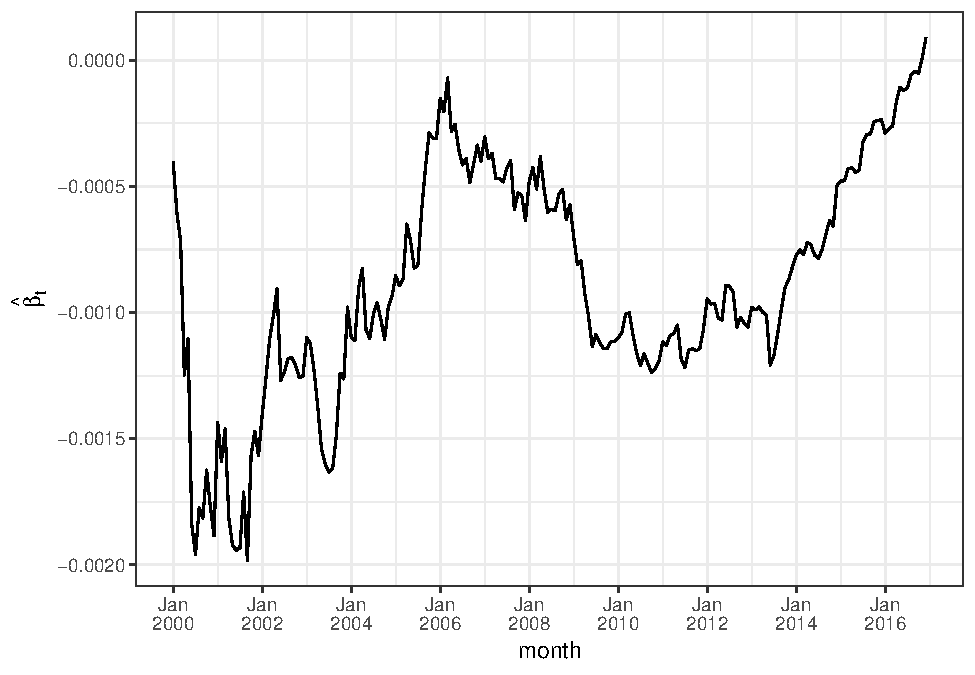
\includegraphics{../figs/freq--trend-growth-1.pdf}
\caption{\label{fig:trend-growth}Filtering estimates of the slope
(\(\beta_t\))}
\end{figure}

\begin{table}[t]

\caption{\label{tab:mape-table}Mean, standard deviation, min and max of prediction errors}
\centering
\begin{tabular}{llrrrr}
\toprule
horizon & model & mean & SD & min & max\\
\midrule
6 & ARIMA & 0.0391 & 0.0108 & 0.0169 & 0.0611\\
 & DLM1 & 0.0427 & 0.0171 & 0.0103 & 0.0689\\
 & DLM2 & 0.0359 & 0.0105 & 0.0163 & 0.0568\\
 & ETS & 0.0366 & 0.0107 & 0.0136 & 0.0573\\
 & Holt-Winters & 0.0438 & 0.0186 & 0.0191 & 0.0743\\
\addlinespace
 & Naïve & 0.0560 & 0.0216 & 0.0207 & 0.0916\\
 & StructTS & 0.0410 & 0.0101 & 0.0215 & 0.0620\\
 & TBATS & 0.0428 & 0.0081 & 0.0251 & 0.0599\\
12 & ARIMA & 0.0514 & 0.0168 & 0.0294 & 0.0833\\
 & DLM1 & 0.0577 & 0.0264 & 0.0233 & 0.1029\\
\addlinespace
 & DLM2 & 0.0429 & 0.0096 & 0.0295 & 0.0733\\
 & ETS & 0.0453 & 0.0162 & 0.0241 & 0.0744\\
 & Holt-Winters & 0.0605 & 0.0271 & 0.0256 & 0.1051\\
 & Naïve & 0.0537 & 0.0143 & 0.0352 & 0.0800\\
 & StructTS & 0.0534 & 0.0154 & 0.0332 & 0.0774\\
\addlinespace
 & TBATS & 0.0528 & 0.0158 & 0.0299 & 0.0911\\
18 & ARIMA & 0.0619 & 0.0266 & 0.0283 & 0.1113\\
 & DLM1 & 0.0756 & 0.0411 & 0.0340 & 0.1524\\
 & DLM2 & 0.0491 & 0.0096 & 0.0357 & 0.0786\\
 & ETS & 0.0526 & 0.0226 & 0.0254 & 0.0963\\
\addlinespace
 & Holt-Winters & 0.0795 & 0.0376 & 0.0304 & 0.1473\\
 & Naïve & 0.0573 & 0.0149 & 0.0355 & 0.0884\\
 & StructTS & 0.0663 & 0.0241 & 0.0344 & 0.1060\\
 & TBATS & 0.0610 & 0.0277 & 0.0298 & 0.1362\\
\bottomrule
\end{tabular}
\end{table}

\section*{Bibliography}\label{bibliography}
\addcontentsline{toc}{section}{Bibliography}

\hypertarget{refs}{}
\hypertarget{ref-bergmeir2012use}{}
Bergmeir, Christoph, and José M Benítez. 2012. ``On the Use of
Cross-Validation for Time Series Predictor Evaluation.''
\emph{Information Sciences} 191. Elsevier: 192--213.

\hypertarget{ref-bergmeir2018}{}
Bergmeir, Christoph, Rob J. Hyndman, and Bonsoo Koo. 2018. ``A Note on
the Validity of Cross-Validation for Evaluating Autoregressive Time
Series Prediction.'' \emph{Computational Statistics \& Data Analysis}
120: 70--83.
doi:\href{https://doi.org/https://doi.org/10.1016/j.csda.2017.11.003}{https://doi.org/10.1016/j.csda.2017.11.003}.

\hypertarget{ref-canova1998detrending}{}
Canova, Fabio. 1998. ``Detrending and Business Cycle Facts.''
\emph{Journal of Monetary Economics} 41 (3). Elsevier: 475--512.

\hypertarget{ref-durbin2012time}{}
Durbin, James, and Siem Jan Koopman. 2012. \emph{Time Series Analysis by
State Space Methods}. Oxford university press.

\hypertarget{ref-hamilton2018}{}
Hamilton, James D. 2018. ``Why You Should Never Use the Hodrick-Prescott
Filter.'' \emph{Review of Economics and Statistics} 100 (5). MIT Press:
831--43.

\hypertarget{ref-holt2004forecasting}{}
Holt, Charles C. 2004. ``Forecasting Seasonals and Trends by
Exponentially Weighted Moving Averages.'' \emph{International Journal of
Forecasting} 20 (1). Elsevier: 5--10.

\hypertarget{ref-hyndman2018forecasting}{}
Hyndman, Rob J, and George Athanasopoulos. 2018. \emph{Forecasting:
Principles and Practice}. OTexts.

\hypertarget{ref-hyndman2019}{}
Hyndman, Rob J, and Yeasmin Khandakar. 2008. ``Automatic Time Series
Forecasting: The Forecast Package for R.'' \emph{Journal of Statistical
Software} 26 (3): 1--22.
\url{http://www.jstatsoft.org/article/view/v027i03}.

\hypertarget{ref-hyndman2002state}{}
Hyndman, Rob J, Anne B Koehler, Ralph D Snyder, and Simone Grose. 2002.
``A State Space Framework for Automatic Forecasting Using Exponential
Smoothing Methods.'' \emph{International Journal of Forecasting} 18 (3).
Elsevier: 439--54.

\hypertarget{ref-kalman1960contributions}{}
Kalman, Rudolf Emil, and others. 1960. ``Contributions to the Theory of
Optimal Control.'' \emph{Bol. Soc. Mat. Mexicana} 5 (2): 102--19.

\hypertarget{ref-kaplan2017understanding}{}
Kaplan, Greg, and Sam Schulhofer-Wohl. 2017. ``Understanding the
Long-Run Decline in Interstate Migration.'' \emph{International Economic
Review} 58 (1). Wiley Online Library: 57--94.

\hypertarget{ref-monahan1984note}{}
Monahan, John F. 1984. ``A Note on Enforcing Stationarity in
Autoregressive-Moving Average Models.'' \emph{Biometrika} 71 (2). Oxford
University Press: 403--4.

\hypertarget{ref-mulder2018putting}{}
Mulder, Clara H. 2018. ``Putting Family Centre Stage: Ties to
Nonresident Family, Internal Migration, and Immobility.''
\emph{Demographic Research} 39. JSTOR: 1151--80.

\hypertarget{ref-petris2009dynamic}{}
Petris, Giovanni, Sonia Petrone, and Patrizia Campagnoli. 2009.
\emph{Dynamic Linear Models with R}. Springer.

\hypertarget{ref-tashman2000out}{}
Tashman, Leonard J. 2000. ``Out-of-Sample Tests of Forecasting Accuracy:
An Analysis and Review.'' \emph{International Journal of Forecasting} 16
(4): 437--50.
doi:\href{https://doi.org/https://doi.org/10.1016/S0169-2070(00)00065-0}{https://doi.org/10.1016/S0169-2070(00)00065-0}.

\hypertarget{ref-teriele2019}{}
te Riele, Saskia, Huisman Corina, Lenny Stoeldraijer, Andries de Jong,
Coen van Duin, and Trond Husby. 2019. ``PBL/Cbs Regionale Bevolkings-
Enhuishoudensprognose 2019--2050: Belangrijkste Uitkomsten.''
\emph{Statistische Trends}. CBS.

\hypertarget{ref-winters1960forecasting}{}
Winters, Peter R. 1960. ``Forecasting Sales by Exponentially Weighted
Moving Averages.'' \emph{Management Science} 6 (3). INFORMS: 324--42.

\hypertarget{ref-zietz2014us}{}
Zietz, Joachim, and Anca Traian. 2014. ``When Was the Us Housing
Downturn Predictable? A Comparison of Univariate Forecasting Methods.''
\emph{The Quarterly Review of Economics and Finance} 54 (2). Elsevier:
271--81.


\end{document}
